\documentclass[serif]{beamer}

\usetheme{CambridgeUS}
\usecolortheme{dolphin}

\usepackage{bm,color}
\usepackage{graphicx}
%\usepackage[brazil, english]{babel}
\usepackage{mathrsfs,amssymb,amsmath,enumerate}
%\usepackage{tgschola}
\usepackage{verbatim,graphicx,geometry,color}
\usepackage[utf8]{inputenc}
%\usepackage{setspace}
\usepackage{amsthm}

\newtheorem{prop}{Proposition}
%\newtheorem{lemma}{Lemma}[section]
\theoremstyle{definition}


\newcommand{\E}{\mathbb{E}}
\newcommand{\Var}{\mathrm{Var}}
\newcommand{\plim}{\overset{p}{\longrightarrow}}
\newcommand{\dlim}{\overset{d}{\longrightarrow}}

\usepackage{hyperref}
%\hypersetup{
%  colorlinks = true,
%  linkcolor = red!60!black,
%}
%\renewcommand{\thefootnote}{\arabic{footnote}}
%
%\makeatletter
%\let\@mycite\@cite
%\def\@cite#1#2{{\hypersetup{linkcolor=blue!60!black}[{#1\if@tempswa , #2\fi}]}}
%\makeatother


\begin{document}

\title[Combinatorial Growth]{Mechanics of Combinatorial Growth: \\ Welfare Results}
\author[Alexandre Sollaci]{Alexandre Sollaci}
\institute[UChicago]{The University of Chicago}
\date{\today}

\begin{frame}[noframenumbering]
\titlepage
\end{frame}

\frame{\frametitle{Welfare with Original Parameterization}
\begin{itemize}
\item New technology subsidies were usually welfare diminishing.
\item Proposed reason: ``corner solution".
\item Benefit of new technology (around 1.9) was too big compared with cost (weibull($\lambda=1,\kappa=2$)).
\item Subsidies therefore would only very seldom have any positive effect at all.
\item To test: increase $\lambda = 2$ without changing anything else.
\end{itemize}
}

\frame{
\centering
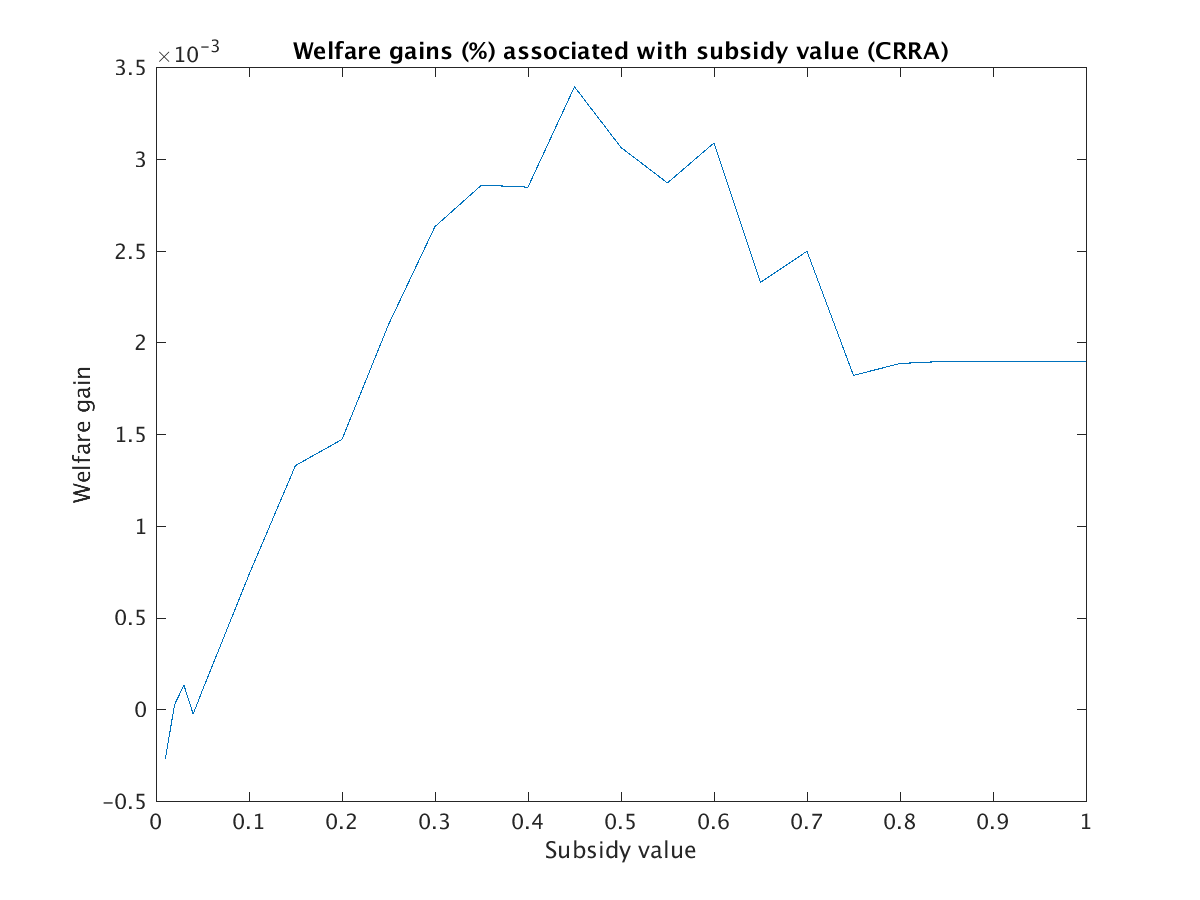
\includegraphics[scale=.6]{figures/welfare_pp_cost2.png}
}

\frame{\frametitle{Welfare with Original Parameterization}
\begin{itemize}
\item Welfare becomes a bell-shaped curve on subsidy.
\item Curiously, optimal welfare brings the model back to the original parameterization.
\item Even a 100\% subsidy still has positive results. The reason is that there is a natural limit on new technologies, which is the probability that inventors come up with them.
\item Also explains why the welfare effect is flat after a 70\% subsidy.
\item However, this is not always the case. If we increase the mode of the idea distribution by 1\% and run the same simulation:
\end{itemize}
}

\frame{
\centering
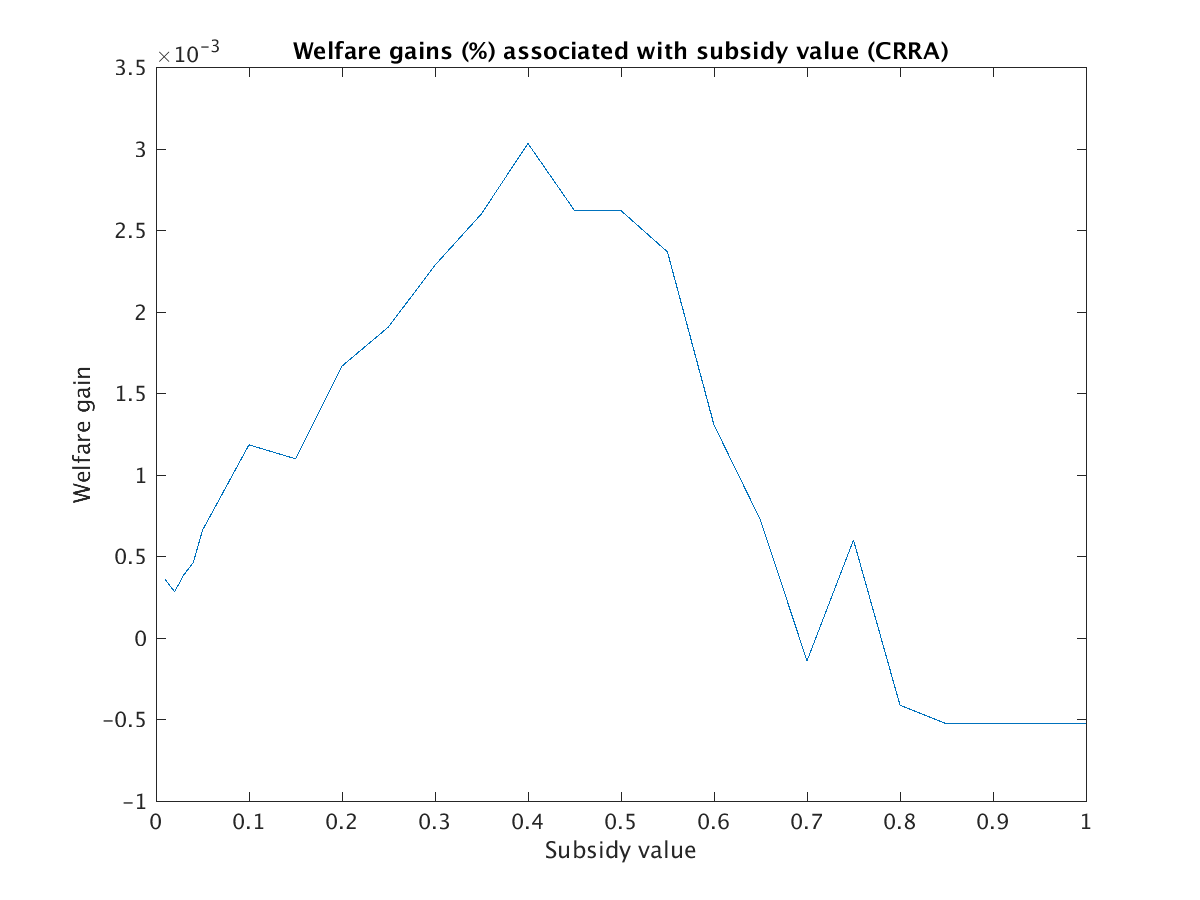
\includegraphics[scale=.6]{figures/welfare_pp_cost01.png}
}

\frame{\frametitle{Escape from Corner Solution}
\begin{itemize}
\item Taking that into account, add an extra parameter to the model, $\phi$.
\item New ideas deistribution is now $g(\phi m, \tau)$ (before $\phi \equiv 1$).
\item Recalibrate the model to fit patent fraction distributions over time (I did it crudely and by hand).
\item Keep a higher cost, $\lambda = 2$ but with $\phi = 1.075$. 
\item Other values changed: $\xi = 5$, $\tau = 500$, $\eta^M = 0.1$.
\end{itemize}
}

\frame{\frametitle{Moment Matching}
\centering
\begin{tabular}{|l|l|l|}
\hline
&\textbf{Data}&\textbf{Model}\\\hline
\textbf{new tech 1850}&0.4&0.10921\\\hline
\textbf{new comb 1850}&0.25&0.25847\\\hline
\textbf{reuse 1850}&0.35&0.63232\\\hline
\textbf{new tech 1900}&0.03&0.036378\\\hline
\textbf{new comb 1900}&0.45&0.43172\\\hline
\textbf{reuse 1900}&0.52&0.5319\\\hline
\textbf{new tech 1950}&0.02&0.029526\\\hline
\textbf{new comb 1950}&0.75&0.76079\\\hline
\textbf{reuse 1950}&0.33&0.20968\\\hline
\textbf{new tech 2000}&0.01&0.0297\\\hline
\textbf{new comb 2000}&0.8&0.80735\\\hline
\textbf{reuse 2000}&0.19&0.16295\\\hline
\textbf{reuse peak}&0.55&0.65927\\\hline
\end{tabular}
}

\frame{
\centering
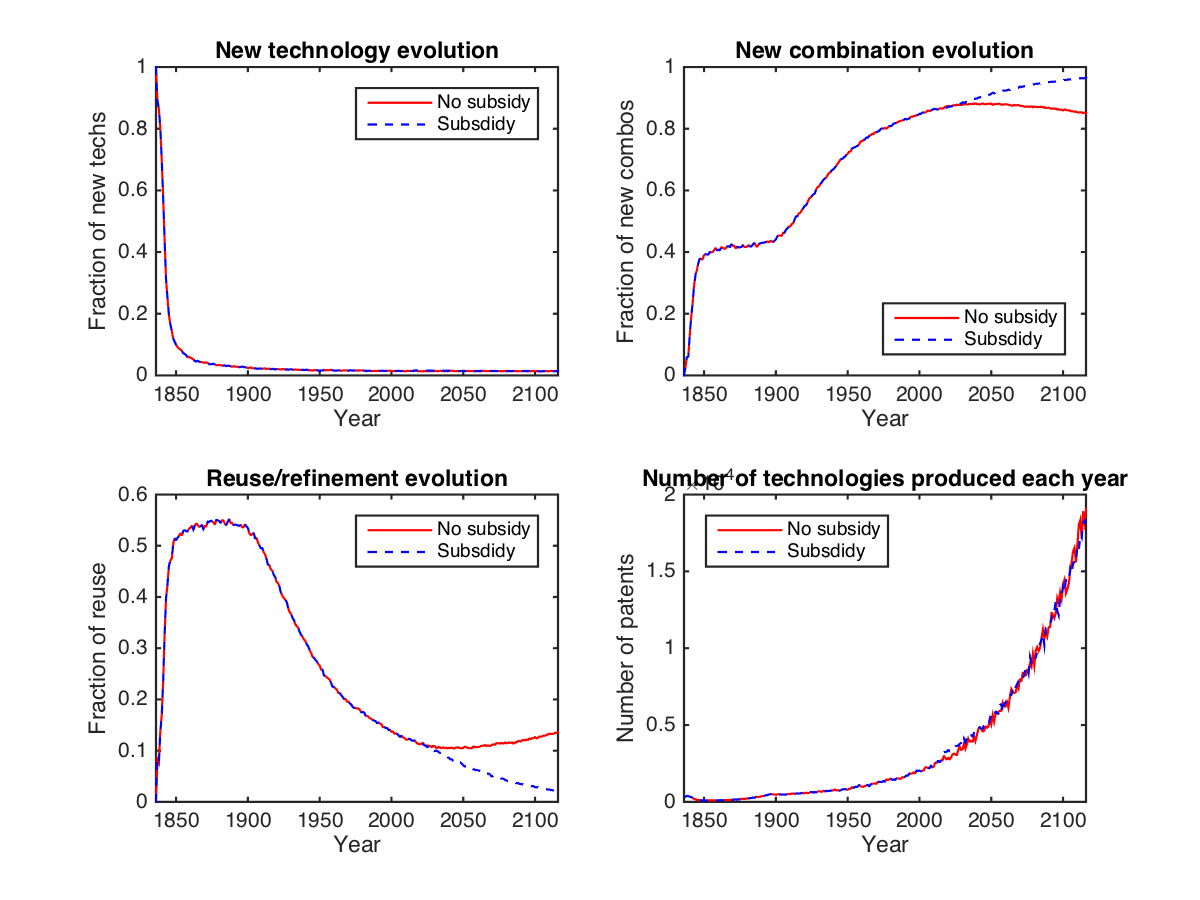
\includegraphics[scale=.6]{figures/patents.png}
}

\frame{\frametitle{Results from Optimal Subsidy}
\begin{itemize}
\item Optimal subsidy has a inverted-U shape, but with a much lower peak.
\item Also try subsidy for new combinations (alone) and all ideas.
\item New combinations subsidy does a much better job to increase welfare: it still has the externality of getting product lines to become hot, but it is a much higher fraction of patents, with a larger potential for influencing the mean quality of goods.
\end{itemize}
}

\frame{
\centering
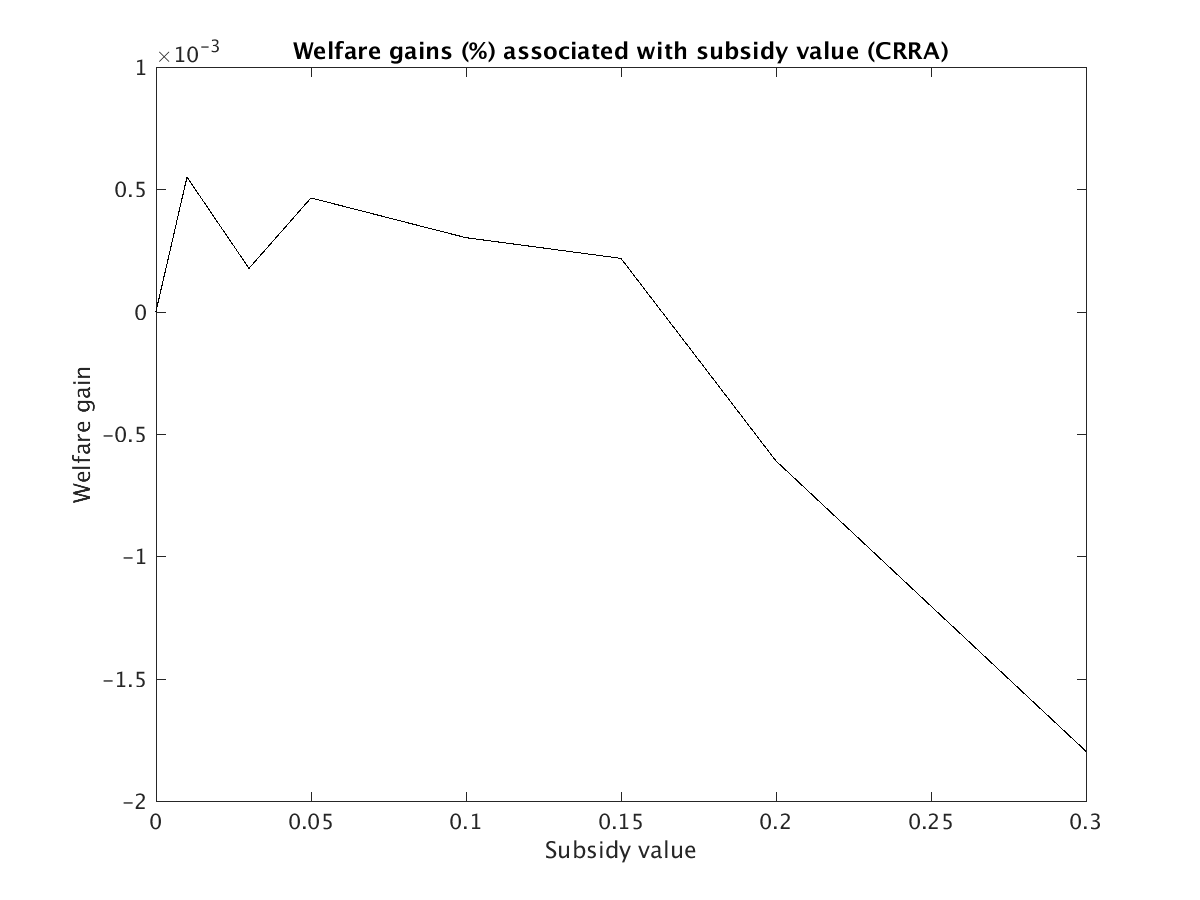
\includegraphics[scale=.6]{figures/welfare_pp_NT.png}
}

\frame{
\centering
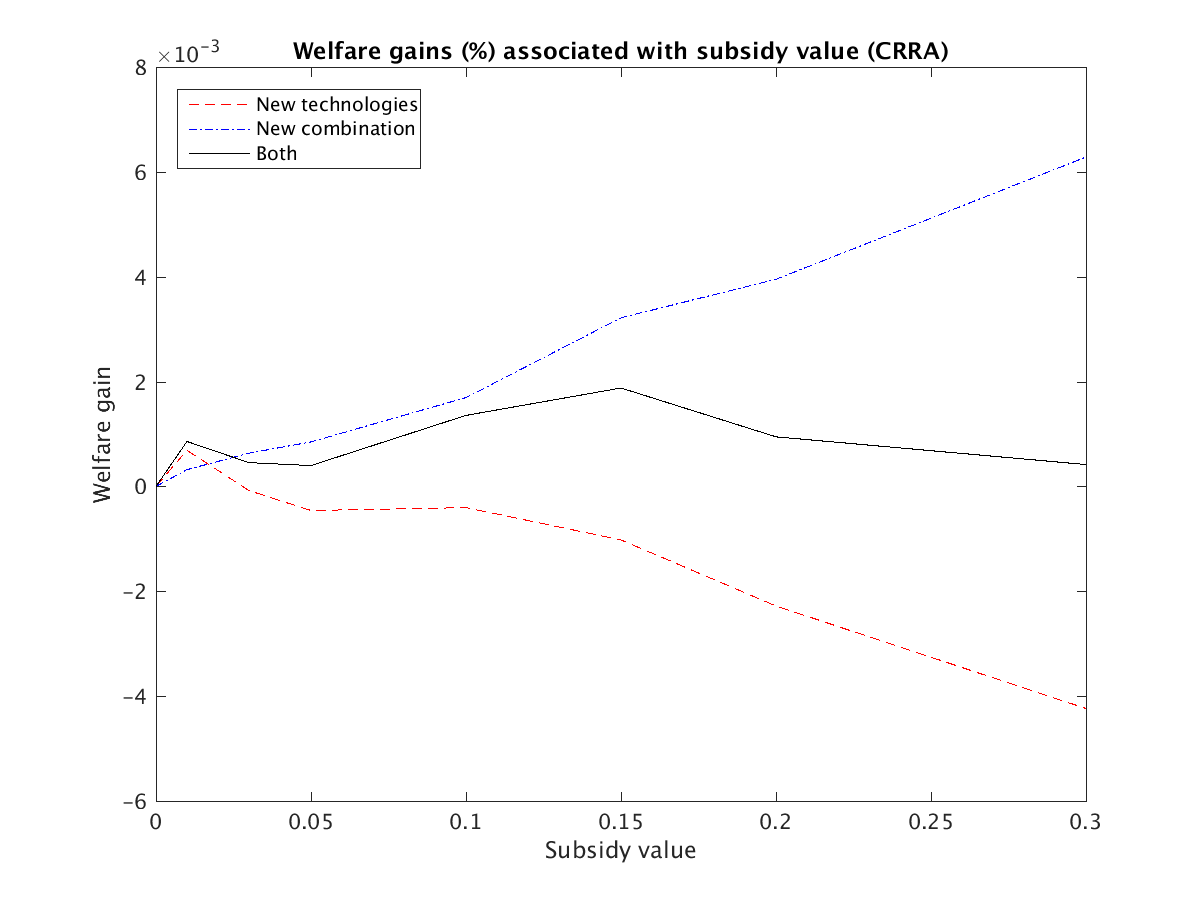
\includegraphics[scale=.6]{figures/welfare_pp_phi_3ways.png}
}

\frame{\frametitle{Thoughts}
\begin{itemize}
\item The fact that the new combination subsidy has better results than the new technologies subsidy is surprising; but it also makes sense.
\item New combinations are the majority of patents, so a subsidy on new combinations would increase the quality of goods by much more than new technologies ever could (and mostly at the expense of reuses, I think).
\item New combinations also have the same externality as new technologies, which is to make product lines hot.
\item Interesting conclusion from model: even though it is getting harder and harder to create new technologies, and this could have bleak consequences for growth, the economic growth in the past 50 years or so has been driven by new combinations instead of new technologies.
\item And the possibilities for new combinations only tend to increase, while the chance of creating new technologies only tends to decrease.
\end{itemize}
}


\end{document}